\chapter{Hyperparameters}
\section{K-Means}
For selecting the appropriate amount of clusters, we used an "elbow" plot in combination with the silhouette score.
\begin{enumerate}
  \item Seeds dataset: 4 clusters (see figure: \ref{hyperparameters:k-means-dataset1})
  \item Heart dataset: TODO
\end{enumerate}
\begin{figure}
  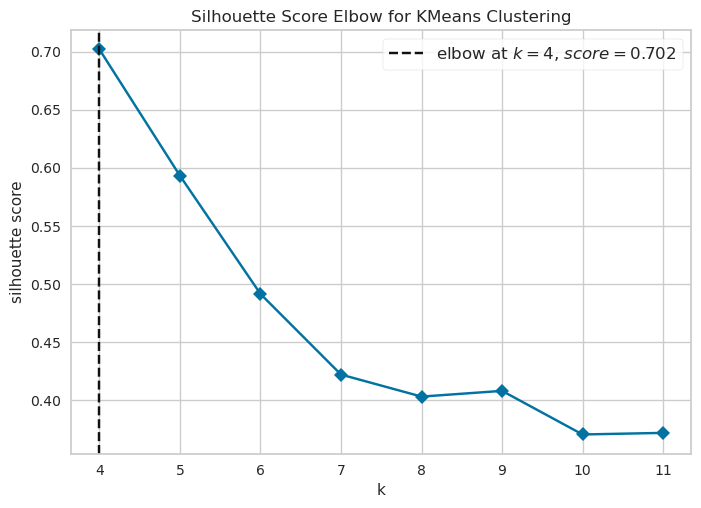
\includegraphics{Appendix/parameter-selection/selecting-k.png}
  \caption{Selecting the $k$ for K-Means for dataset 1 using the "elbow plot" using section \ref{theory:kmeans}}
  \label{hyperparameters:k-means-dataset1}
\end{figure}